\chapter{Variance in Vision Models: a Convolutional Sparse Coding Approach}

\begin{flushright}
    \textit{''These stats are staggering \\
    Had his Ph.D in indiscreet street haggling.''} \\
    MF Doom, Gazzillion Ear, 2009

    %\textit{''The proof of the pudding is in the eating.''}\\
    %British proverb
\end{flushright}

%\begin{flushright}
%    \textit{''As far as the laws of mathematics refer to reality, they are not certain;\\
%    and as far as they are certain, they do not refer to reality.''}\\
%    Albert Einstein, Lecture at the Prussian Academy of Science in Berlin, 1921
%\end{flushright}

\chaptertoc{}

\section{Introduction: Orientation, Statistics, and Orientation Statistics}
As introduced in the previous chapter, a central role of the brain is to build a model of its environment in order to enact complex behaviors. One key component of these models is their reliance on internal representations of the environment. While this is true in predictive coding (where these representations are predictions), it also forms the dominant narrative in neuroscience~\cite{keller2018predictive}. This understanding of the brain stems from the discovery of the receptive field, by Sherrigton's seminal studies~\cite{sherrington1906observations}, which correlated a neural discharge pattern with an element of the environment (here, stroking a certain skin spot). Iteration upon iteration of related research have built modern neuroscience upon a similar narrative, starting with the "fly detectors" neurons of Barlow~\cite{barlow1956retinal}, the orientation selective neurons of Hubel and Wiesel~\cite{hubel1959receptive}, the place cells of O'Keefe and Dostrovsky~\cite{o1971hippocampus}, the grid cells of Hafting~\cite{hafting2005microstructure}, the face cells of Perret~\cite{perrett1982visual}, and so on~\cite{martin1994brief}. 

In vision, there is thus no denying that orientation forms the basis of these models of the world internalized in the brain. One legitimate question that should be asked before diving into $4$ chapters of studies related to orientation selectivity could be: "why orientations in the first place" ? As history would have it, Hubel and Wiesel discovery was somewhat serendipitous~\cite{martin1994brief}, and orientation selectivity was discovered somewhat accidentally when the two scientists noticed strong neural responses as they were inserting a glass slide (used to project the spots of light) into the projector of their cat experiments. It thus become evident that neurons in \gls{V1} were in fact responding not to spots of light, as in the retina and \gls{LGN}, but to the edge of the glass slide, indicating a selectivity for oriented edges. 

Had computational neuroscience been $30$ years more advanced at the time of these experiments, Hubel and Wiesel might have had the chance of knowing what to look for in the first place, rather than stumble upon it semi-accidentally. Indeed, we have said that a key property of the brain is efficient coding~\cite{barlow1961possible}, which saves costly neurobiological message passing by encoding solely relevant information. Under predictive coding, for example, this means solely transmitting prediction errors. This generic principle imposes a constraint of sparseness on the message to be sent by neurons, meaning using as little energy as possible while maintaining a highly accurate internal model. Thus, one can envision early sensory cortices as models of the world build through the transformation of dense redundant inputs into sparse efficient representations. By creating a computer model that performs high-quality reconstruction with as little activity as possible, one can thus see what types of features are ideal to deconstruct any given type of sensory input. This trade-off has been explored by Olshausen and Field~\cite{olshausen1996emergence}, who showed that a model of natural images with a constraint of sparsity yields receptive fields that are extremely similar to those found in \gls{V1} (Figure~\ref{fig_chap3_olshausen}). Thus, a low-level invariant representation of the (static) visual world can be created using edges detector.

\begin{figure}[h!tbp]
\vspace{0.1cm}
\centering
\includegraphics[width=1.\textwidth]{fig/chap3_olshausen.pdf}
\caption[Natural images and sparse dictionaries.]{Natural images and sparse dictionaries. 
(left) Natural images components, extracted using Principal Component Analysis (PCA). 
(middle) Dictionaries yielded by learning a sparse code on natural images, from~\cite{olshausen1996emergence}. 
(right) Comparison with macaque \gls{V1} receptive fields, from~\cite{ringach2002orientation}.}
\label{fig_chap3_olshausen}
\end{figure}

The statistical distribution of these edges in any given image follows a characteristic pattern~\cite{perrinet2015edge}, and given optimal modelling, these statistics are the main constraint upon which further sensory processing relies~\cite{olshausen1997sparse}. Most of these oriented edges are represented at the cardinals points, that is, horizontally and vertically~\cite{coppola1998distribution}. This is echoed at the neuronal level by a cardinal bias in visual perception~\cite{hansen2004horizontal}. As we will show in this chapter's article, around either of these main orientations, the distribution of oriented elements can be characterized by its first- and second-order moments: a median orientation, and its corresponding (inverse) variance. A proper model of a natural images thus depends on a proper model of both these moments (Figure~\ref{fig_chap3_ori_distrib}), which is reflected in the response properties of primary visual cortex neurons that have diverse orientation and variance~\cite{hubel1962receptive}. 

\begin{figure}[h!tbp]
\vspace{0.1cm}
\centering
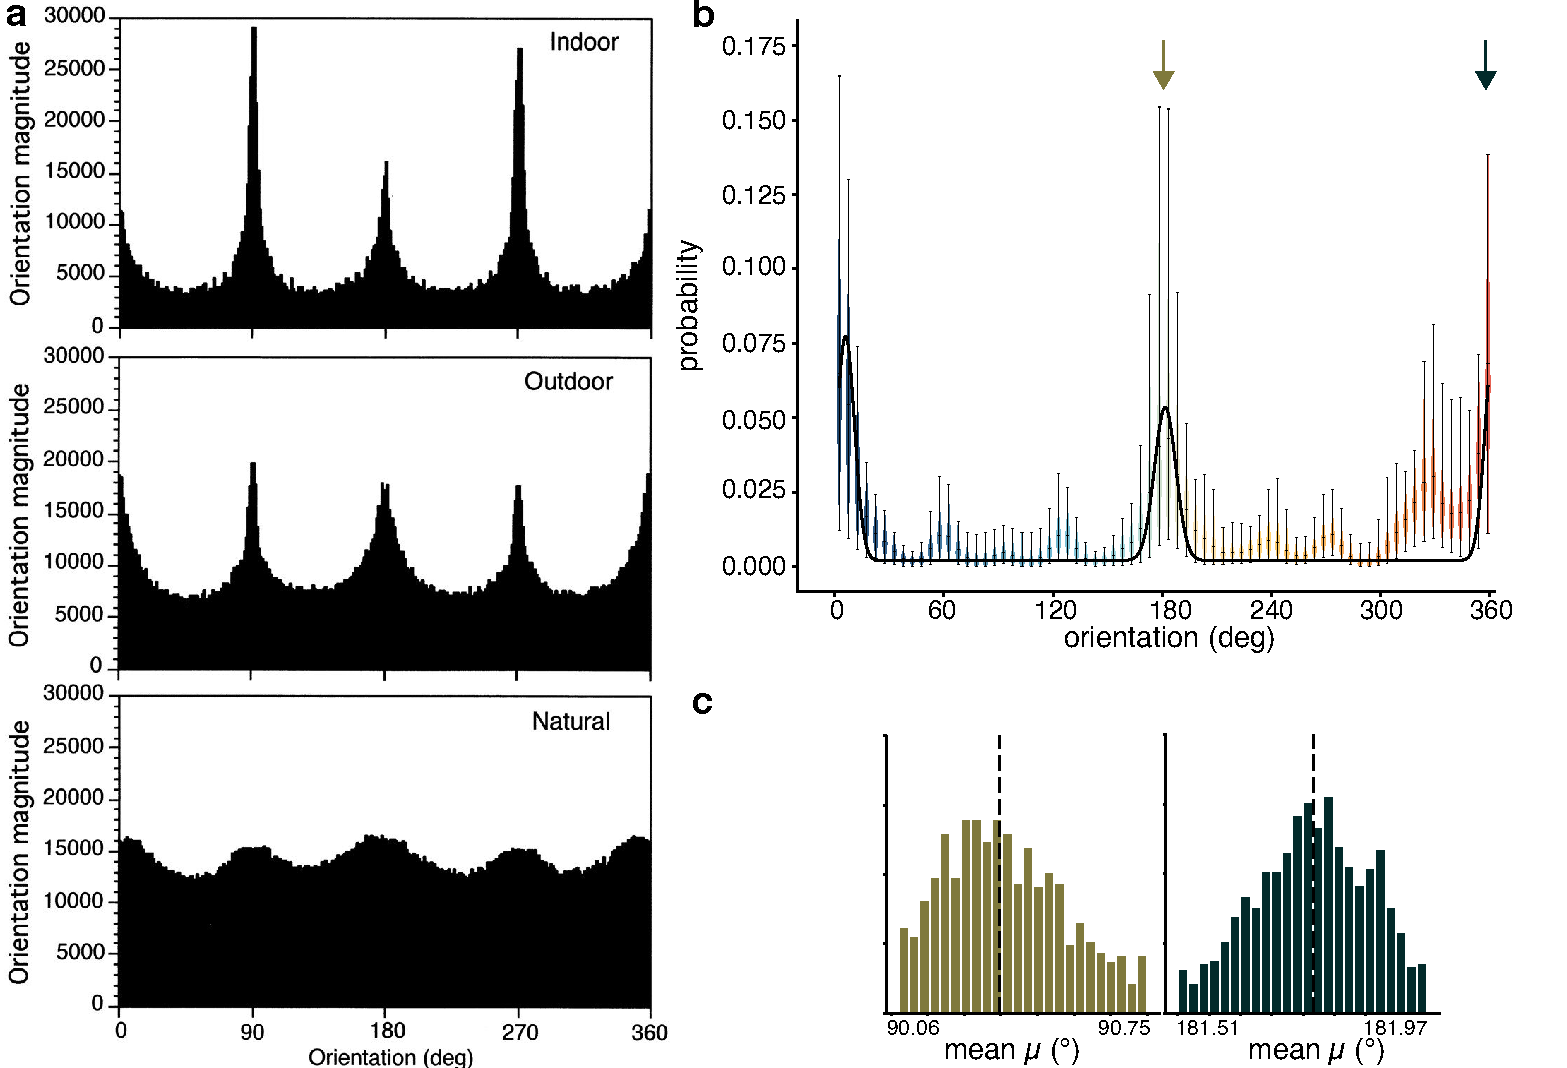
\includegraphics[width=1.\textwidth]{fig/chap3_ori_distrib.pdf}
\caption[Distribution of orientations in natural images.]{Distribution of orientations in natural images.
(a) Distribution of oriented contours, extracted by Sobel filters (see this chapter's article), as done in~\cite{coppola1998distribution}. 
(b) Distribution of oriented contours, extracted by Sparse Coding (as done in this chapter's article), with mean von Mises distribution in black. 
(c) Distribution of means of two peaks of the distributions, for each image.}
\label{fig_chap3_ori_distrib}
\end{figure}

If orientations in natural images follow such a prototypical distribution, then what is the optimal neural code to represent them ? This question is one of uncertainties. Uncertainty on how the image's orientation deviates from the typical distribution is a problem of uncertainty bound to the input, called aleatoric uncertainty. Uncertainty on how to best model these images is a problem of uncertainty bound to the model, referred to as epistemic uncertainty. Aleatoric uncertainty is linked to the variance of the distribution of orientation: the higher the variance, the more spread the input is (in orientation space), and thus the less certain the information is. As stated in the introduction, linking this aleatoric uncertainty/variance to the uncertainty of the model is crucial for Bayesian processing, which provides explicit rules to do so (see Equation~\ref{eq_proba_intro}). 

This chapter serves to characterize natural images as Gaussian (or here, von-Mises) distributions of oriented features, which allows us to keep working within the mathematical framework described in the introduction. This further serves as a justification of Gaussian distribution of orientation as stimuli for animal recordings in chapter 4. Second, it serves to understand how the variance of natural images can be processed by a model with no explicit learning rules for variance. This, again, is useful to describe variance interactions as an emergent property throughout this thesis. Third, as we'll delve into in this chapter's conclusion, this perspective enables us to examine the trade-off between two encoding strategies. One approach involves dense sampling using numerous neurons, providing high quality reconstruction but at a higher energy cost. The alternative employs sparse sampling, where fewer neurons co-encode features and their variance. Under the right conditions, this latter strategy can be equally performant, but much more energy-efficient.

\section{Methods: Sparse Coding}
\begin{figure}[h!tbp]
\vspace{0.1cm}
\centering
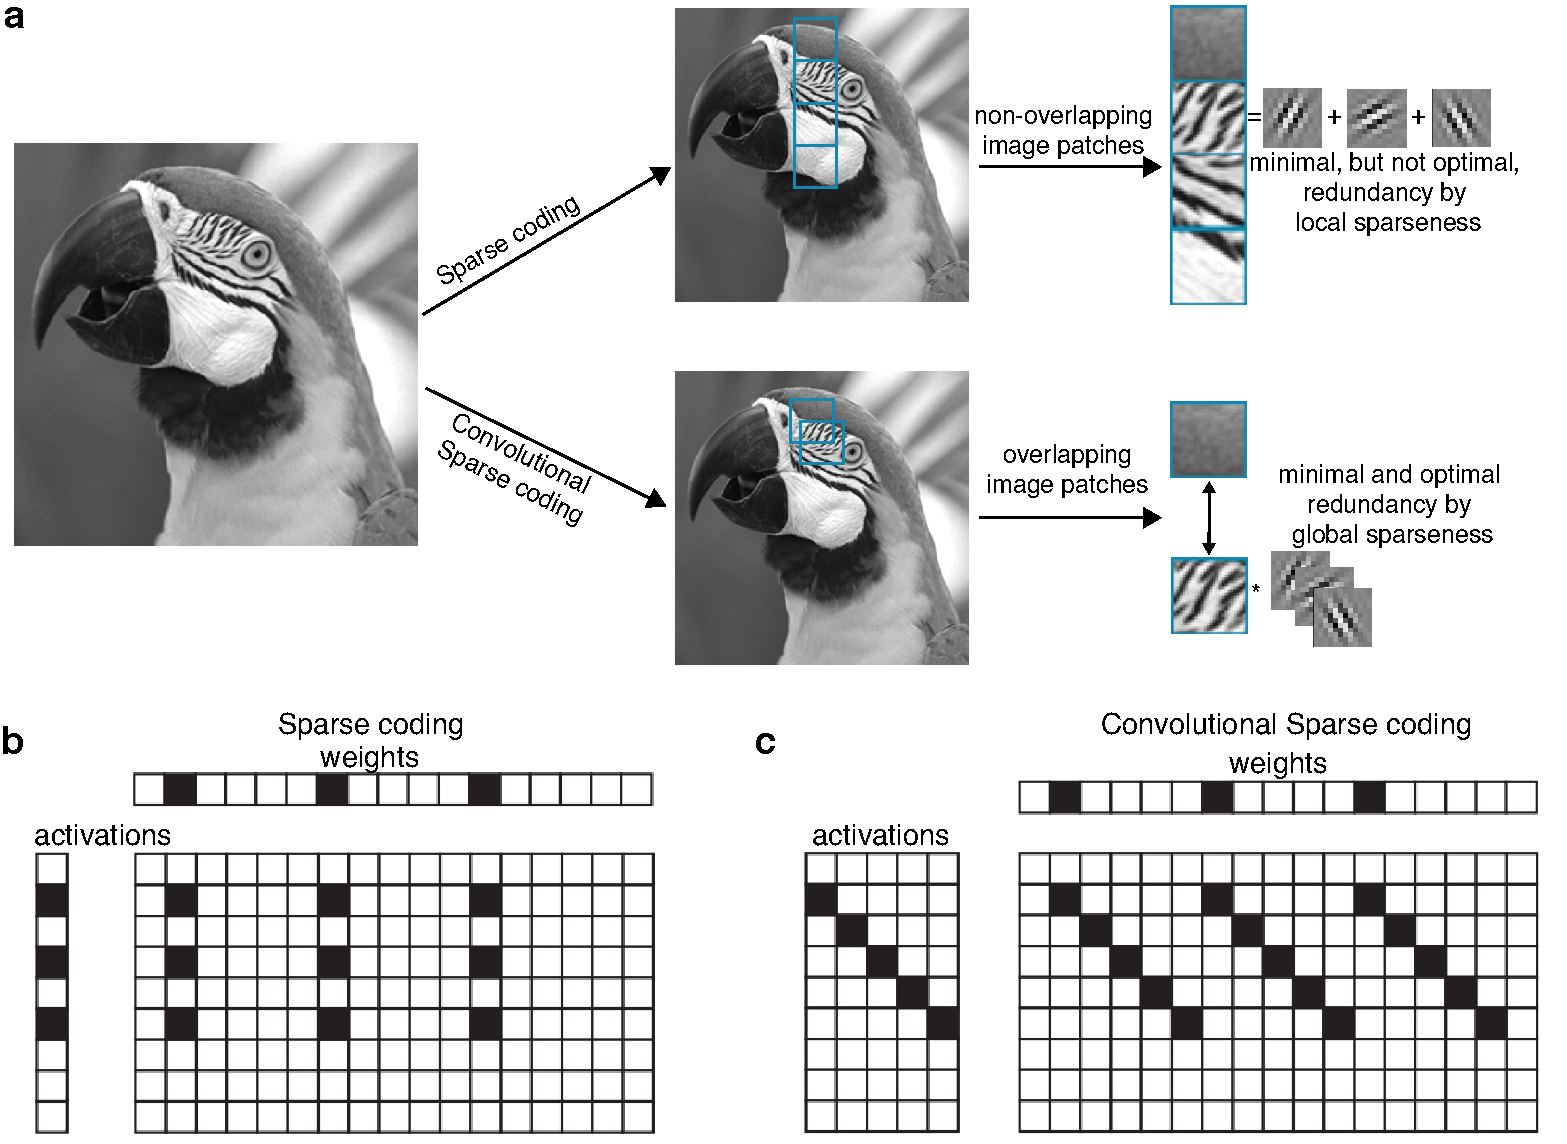
\includegraphics[width=1.\textwidth]{fig/chap3_csc.pdf}
\caption[Convolutional Sparse Coding.]{(a) Convolutional Sparse Coding (bottom) relies on convolution operations to achieve global sparseness and remove local redundancies (top), mimicking the operation of the visual system. (b) and (c), visualized as vector-vector or vector-matrix products.}
\label{fig_chap3_csc}
\end{figure}

The model used by Olshausen and Field~\cite{olshausen1996emergence} to show the emergence of orientation selectivity in sparsely-constrained algorithm is referred to as Sparse Coding (SC), and is a widely used model for learning the inverse representation of an input signal. Given the assumption that a signal can be represented as a linear mixture of basis functions (in neurobiological terms, receptive fields), the optimization problem solved by sparse coding is one that tries to minimize the number of basis functions that are used to represent the input signal (which would be spikes), yielding a compact and efficient representation of the original signal. Here, we framed sparse coding as the problem of reconstructing an image $s$ from sparse representations $x$ while minimizing a $\text{L}_1$ norm of the representation. This problem can be approached with a Basis Pursuit DeNoising (BPDN) algorithm:
\begin{equation} 
    \underset{x}{\operatorname{arg min}} \frac{1}{2} || s - D x ||^2_2 + \lambda ||x ||_1
\end{equation} 
where $D$ is a dictionary (i.e. a set of basis functions used to represent $s$) and $\lambda$ a regularization parameter that controls the trade-off between fidelity and sparsity. The present article uses a variation of sparse coding, Convolutional Sparse Coding (CSC), which, as the name implies, relies on the convolution operator: 
\begin{equation} \label{eq:csc}
    \underset{\{x_k\}}{\operatorname{arg min}} \frac{1}{2}
    || s - \sum_{k=1}^K \text{d}_k \ast x_k ||^2_2 + 
    \lambda \sum_{k=1}^K ||x_k||_1
\end{equation}
where $x_k$ is an $N^2$ dimensional coefficient map (given an $N^2$ sized image), $\text{d}_k$ is one kernel (among $K$ channels) and $\ast$ is the convolution operator (Figure~\ref{fig_chap3_csc}). One additional advantage of convolutional sparse coding over other reconstruction techniques is its ability to learn interpretable features from the data, which can be easily visualized and understood by human experimenters~\cite{boutin2020sparse}. 

\section{Methods: Deep Learning}
The final section of this article uses a Deep Neural Network, as a model to understand how the sparse code can be of use in further stage of visual hierarchical processing. While they are not used elsewhere in this thesis, a brief introduction can be useful. All modern artificial neural networks rely on the gradient descent algorithm, as introduced by Rumelhart~\cite{rumelhart1986learning}. The essence of this optimizer is to iteratively adjust the parameters of a neural network to minimize a loss function, defined as the difference between its predictions and the actual data.

Given this loss function \(L(\theta)\), where \(\theta\) represents the parameters of the network, the gradient descent update rule is expressed as:
\begin{equation}
\theta_{t+1} = \theta_t - \alpha \nabla L(\theta_t)
\end{equation}
where \(\theta_{t+1}\) is the updated parameter at iteration \(t+1\), \(\alpha\) is the learning rate, and \(\nabla L(\theta_t)\) is the gradient of the loss with respect to the parameters at iteration \(t\).

Here, we use a Convolutional Neural Network, as introduced by LeCun et al.~\cite{lecun1998gradient} to demonstrate the capability of learning hierarchical features is a central model in Deep Learning for processing grid-like topology data, such as images. This model is based on the idea that an input signal can be represented through a hierarchical set of layers, where each layer transforms the input data with the aim of gradually abstracting the features of the data to enable effective classification or regression at the output layer.

Given an input image \(I\), a Convolutional Neural Network seeks to learn a hierarchy of convolutional features \(F\) by applying a series of convolutional and pooling operations, typically defined as:
\begin{equation}
F_l = \operatorname{ReLU}(W_l \ast F_{l-1} + b_l)
\end{equation}
where \(F_l\) is the feature map at layer \(l\), \(W_l\) is the convolutional kernel, \(b_l\) is the bias term, and \(\ast\) is the convolution operator.

Deeper architectures, that is, with more layers, also contain a MaxPooling operation which groups representations into an intermediate, dense form: 
\begin{equation}
F_{\text{deep}} = \operatorname{MaxPooling}(\operatorname{ReLU}(W_{\text{deep}} \ast F_{\text{prev}} + b_{\text{deep}}))
\end{equation}
where \(F_{\text{deep}}\) represents the deeply learned features, and \(F_{\text{prev}}\) is the feature map from the previous layer. These Deep Convolutional Neural Networks, with their deep architectures, have an advantage over other models due to their capability to learn more abstract and generalized representations of input data, which are critical for solving complex problems in computer vision~\cite{krizhevsky2012imagenet}. In this study, we leverage this capability to understand how the representation power of deep layers influences the performance of the model. Each DCNNs has its particular architectural tweaks, for which we would refer the reader to the article in the next section.

\section{Article: "Sparse Representation of Natural Images with Heterogeneous Orientation Kernels"}
The following article is the initial contribution of this thesis, framing natural images as Gaussian-like distribution of oriented elements. This alleviates major non-linear integration difficulties that would otherwise be present in the predictive coding framework, and serves as a justification of the use of Motion Clouds~\cite{leon2012motion} in the next chapter. On its own, the article uses dictionaries of receptive fields that emphasize two coding strategies to reconstruct natural images: focusing either on median features (orientations) or their variance (bandwidths). We show that focusing on the former improves reconstruction, while the latter improves sparseness. Fine-tuning through learning on a dataset of natural images alleviates this compromise, allowing optimal encoding of natural images through a sparse co-encoding strategy, as will be also uncovered in \gls{V1} in chapter 4.  

Full citation is as follows: \fullcite{ladret2023kernel}
% avant d'intégrer un article dans votre thèse, consulter http://www.sherpa.ac.uk/romeo/ si vous souhaitez diffuser sur internet
\includepdfset{pagecommand=\thispagestyle{scrheadings}} % ajoute la numérotation continue des pages aux fichiers pdf importés
\includepdf[scale=1.0,pages=-]{papers/neuralcomp.pdf} % 'scale' ajuste la taille du pdf, vous pouvez affiner en fonction des marges

\section{Conclusion}
Designing an efficient strategy to represent our environment is challenging, especially in a world loaded with statistical variance. Modelling such modelling visual inputs with unpredictable variance is the focal point of this thesis. In the current article, we developed a computational model that learns an optimal representation of natural images, and explored the sparseness/reconstruction trade-off of its receptive fields. By using sparse coding as a way to extract the features necessary to build a representation of natural images, we showed that a neural representation of variance is advantageous, even at the level of Deep Learning research. This ties directly to Bayesian processing, which explicitly derive mathematical rules that integrate both epistemic and aleatoric variances are advantageous (see Equation~\ref{eq_proba_intro}). In contrast, our study concentrates on an implicit emergent encoding of the epistemic and aleatoric variances. This also relates to the idea that computation of variance can be seen as an emergent property, which will be further emphasized in the next chapter. 

A research offspring that will directly stem from this work is to train Deep Neural Networks directly on sparse coefficients that encode an optimal representation of images, rather than images themselves. The preliminary practical work on that end has already been made here, as our codebase in the article consisted of porting a sparse coding library (SPORCO~\cite{wohlberg2017sporco}) into a tensor format~\cite{paszke2017automatic}, allowing for milliseconds-fast computations. Sparse representations, whether here or in the brain, are essentially distributions of binary events weighted by synaptic connectivity. As these Deep Neural Networks relying on spiking activity are set to eventually surpass regular methods~\cite{eshraghian2022memristor, grimaldi2023learning}, there would be great advantage in integrating the work done here in a spiking framework. One final advantageous effect of these sparse representations is their natural property to remove noise in the input. Thus, an encoder that transforms natural images into sparse representations with variance could easily defend against noisy inputs (whether malicious or not), which would prove useful in critical applications such as medical imaging. 

Aside from these machine learning considerations, the key conclusion of this article is the obvious sparseness/reconstruction trade-off involved in encoding natural images, as shown in the first figure of this article, and reproduced in Figure~\ref{fig_chap3_tradeoff}. This emphasizes two possible strategies to encode the distributions of orientation that makes up natural images:
\begin{itemize}
    \item Either a neural system can use multiple orientation-tuned units to encode the full input distribution, at heavy computational and energy costs. This would be equivalent to dense sampling the likelihood $p(u|v)$ (as introduced in Equation~\ref{eq_denominator}).
    \item Or a neural system can use an estimate of orientation and variance, through a receptive field attuned to both of these moments of the distribution. This would then be similar to using a maximum likelihood approach (as introduced in Equation~\ref{eq_MLE}), which means finding the best surrogate function to approximate the distribution in the real input. 
\end{itemize} 
The fact that heterogeneous orientation-tuned functions represent the optimal trade-off for representing natural images will serve as a natural transition towards our next chapter, which will show that \gls{V1} likely implements the first strategy for a fast first estimate, then stabilizes onto the second through recurrent connectivity.

\begin{figure}[h!tbp]
\vspace{0.1cm}
\centering
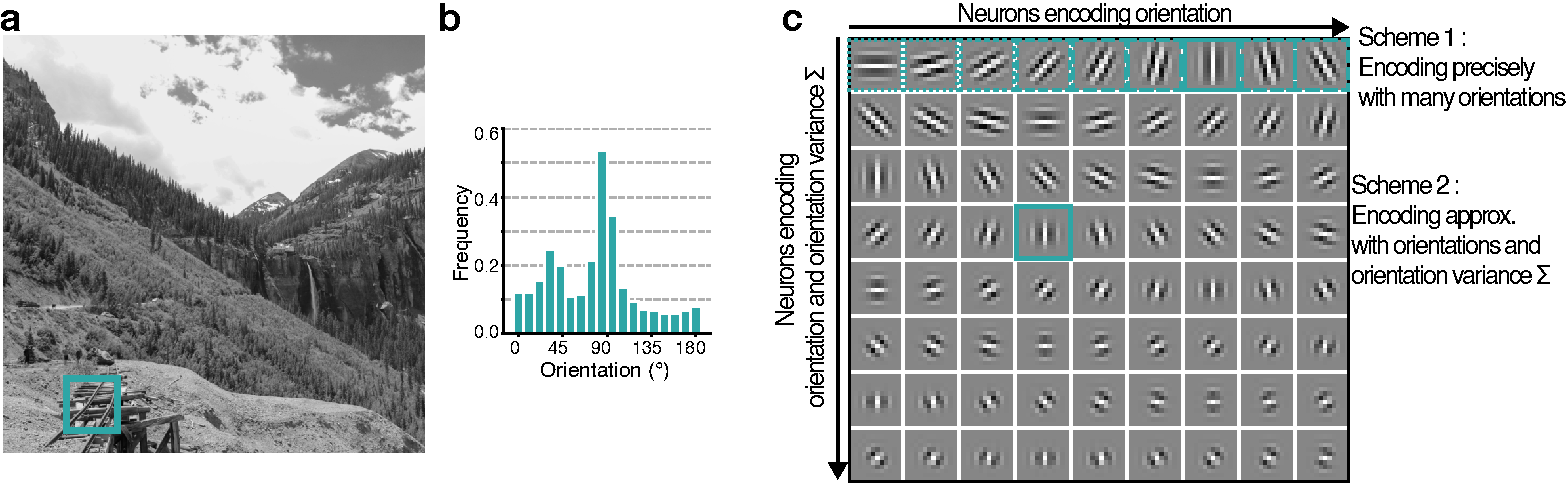
\includegraphics[width=1.\textwidth]{fig/chap3_tradeoff.pdf}
\caption[Sparseness/reconstruction trade-off.]{Sparseness/reconstruction trade-off. (a) A patch of natural image, from the database generated in this article~\cite{ladret2023imgs}. (b) Distribution of orientation from this image, extracted with Sobel filters. (c) Two possible strategies for a neural encoding of this distribution, either through costly but accurate code (Scheme 1) or sparse but less accurate code (Scheme 2).}
\label{fig_chap3_tradeoff}
\end{figure}

This has been preliminarily explored by the Locally Competitive Algorithm, a neuro-inspired algorithm~\cite{rozell2008sparse} which uses recurrent interactions between neurons to drive the sparse coding, as done in Equation~\ref{eq:csc}, but with winner-takes-all competition:
\begin{equation}
    \tau \frac{du_i}{dt} = -u_i + \phi_i - \lambda \sum_{j \neq i} \omega_{ij} \cdot S(u_j) 
\end{equation}
Where \( u_i \) is the internal state (or membrane potential) of neuron \( i \), \( \phi_i \) is the projection of the input onto the \( i^{th} \) basis function (or receptive field), \( \tau \) is a time constant, \( \lambda \) is a positive constant that scales the strength of the competition, \( \omega_{ij} \) represents the degree of overlap or similarity between the receptive fields of neurons \( i \) and \( j \), \( S(u_j) \) is a function that represents the output of neuron \( j \) given its internal state \( u_j \), typically, a threshold function. The design of this algorithm is that neurons compete with each other to represent the input, with neurons that have a dissimilar receptive field competing against one another. Using this Locally Competitive Algorithm as a model of recurrent versus feedforward interactions would also allow seeking which of these two types of connectivity creates the heterogeneous basis functions observed here. It then naturally follows that the next chapter transition from the present functional study, to pinpointing its origin in neurobiological networks.